\mychapter{Credential Relationship Binding Nullifier}

\section{Introduction}

In Chapters 2 and 3, we developed a robust foundation for anonymous credentials, evolving from single-issuer Attribute-Based Anonymous Credentials $(\ABC)$ to the Multi-Issuer Multi-Credential ABC $(\MIMCABC)$ system with identity binding security. $\MIMCABC$ enables users to privately prove that credentials from multiple, mutually distrusting issuers belong to the same identity, a significant advance for applications like federated identity proofs or content credentialing. However, real-world identity systems impose additional requirements that $\MIMCABC$ does not fully address: hierarchical structure and sybil resistance for context-specific credentials.

In practice, credentials often form a natural hierarchy, with foundational identities—such as government-issued IDs or passports—serving as Master Credentials, and dependent credentials—like driver’s licenses, professional certificates, or access rights—acting as Context Credentials. This structure enables efficient revocation: invalidating a Master Credential (e.g., upon employment termination) implicitly revokes all dependent Context Credentials, avoiding the need to track and revoke each individually. Furthermore, regulatory frameworks like KYC/AML demand accountability, requiring systems to prevent sybil attacks where users illegitimately obtain multiple credentials for the same context (e.g., multiple driver’s licenses). 

While MIMC-ABC ensures credentials share a single identity, it lacks mechanisms to enforce this hierarchical dependency or prevent sybil attacks in a privacy-preserving manner, as its identity binding operates agnostically across all credentials without distinguishing their roles or contexts. To meet these practical and regulatory needs, we must extend MIMC-ABC with a cryptographic framework that organizes credentials hierarchically and ensures context-specific uniqueness, all while preserving user anonymity and computational efficiency


\subsection{Problem Statement}

We want to improve MIMC-ABC for real-world use. Our goal is a private credential hierarchy with Sybil resistance. A user has a Master Credential with a secret key $\k$. They also have Context Credentials with unique IDs $\ctx$ (e.g., $\mathcal{H}(\text{"DriverLicense"})$). We need a mechanism that:
\begin{enumerate}
    \item Links each Context Credential to the Master Credential. It uses a unique nullifier $\nul$ from committed values $\k$ and $\ctx$ from different commitments.
    \item Prevents sybil attacks. It prevents multiple nullifiers for the same $(k, \ctx)$ pair.
    \item Verifies nullifier correctness in zero-knowledge. It hides $\k$ and $\ctx$.
\end{enumerate}


Our main challenge is:
\begin{center}
\emph{How do we efficiently generate a verifiable nullifier that proves the binding relationship between two separate credentials without leaking any additional information}
\end{center}

E.g.
\begin{figure}
        \begin{pchstack}[boxed, center, space=4em]
            \begin{pcvstack}
                \procedure[space=auto]{Passport}{%
                \id: 12345, \\
                \ctx: "master", \\
                \exp: "10/11/2026" \\
                \k: 54321
                }
            \end{pcvstack}
            \pcvspace
            \begin{pcvstack}
                \procedure[space=auto]{Driver License}{%
                 \id: 12345, \\
                 \ctx: "DMV", \\
                 \exp: "10/11/2028"
                }
            \end{pcvstack}
            \begin{pcvstack}
                \procedure[space=auto]{Nullifier}{%
                 \textsf{n} = 1/(\k + "DMV") \\
                 \nul = g^{\textsf{n}}
                }
            \end{pcvstack}
        \end{pchstack}
    \caption{Example Credential and Nullifier for context DMV}
    \label{fig:two-creds}
\end{figure}



\subsection{Background Work}

Past works tackled hierarchy and sybil resistance in credential systems. None fully balances privacy, efficiency, and flexibility. 
\begin{enumerate}
    \item The UTT anonymous payment system ~\cite{tomescu2022utt} is the closest work, using a registration credential (like a Master Credential) and the coins are also credentials using serial numbers (like Context Credentials) where a coin can only be spent once. UTT uses pairings in their pseudorandom function which we benchmark against and show our speedup.

    \item CanDID~\cite{maram2021candid} defines Master and Context Credentials clearly, but has weakened privacy. It uses mappings between credential public keys in a table, breaking unlinkability. It also relies on an MPC-based PRF for sybil resistance. This adds complexity and overhead, unfit for lightweight use.

    \item Other pairing-based systems, like SyRA~\cite{crites_syra_2024} and S3ID~\cite{rabaninejad_attribute-based_2024}, offer private hierarchies. Yet, they suffer from pairing-related efficiency issues and slower zero-knowledge proofs where we use $\Sigma$-protocols, which are the most efficient zero-knowledge proofs.

    \item Standard Verifiable Random Functions  (VRFs)~\cite{hutchison_verifiable_2005} reveal the user’s public key during verification impacting anonymity and furthermore are constructed with bilinear pairings.

\end{enumerate}

Our MIMC-ABC system (Chapter 3) binds identities efficiently and anonymously but without hierarchy and context-specific sybil resistance. We need a solution that keeps MIMC-ABC’s strengths. It must add a light, private way to handle credential hierarchies and sybil resistance.




\subsection{Contributions}

We advance anonymous credential systems by developing a lightweight, pairing-free Verifiable Random Function (VRF) construction optimized for our use-case of hierarchical credential binding and sybil resistance. Our contributions are threefold:

\begin{enumerate}
        \item \textbf{Pairing-Free VRF in Prime-Order Groups:} We adapt the Dodis-Yampolskiy VRF structure for standard prime-order groups by replacing the proof mechnaism and prove our construction retains the security properties - \emph{pseudorandomness, uniqueness, verifiability} - under the $q$-DDHI assumption. (We show the efficiency speedup of this change)

        \item \textbf{Novel $\Sigma$-protocols for Inverse Exponents and Committed Inverse Exponents} We develop novel zero-knowledge proof protocols to prove knowledge of an inverse exponent and committed inverse exponent.        
        We use these protocols to prove the correctness of the Diffie Hellman Inversion (DHI) structure used in our Pairing-Free DY VRF VRF. Both techniques are new general techniques for $\Sigma$-protocols.
        
        \item \textbf{Credential Relationship Binding Nullifier } We combine our VRF improvement with our novel $\Sigma$-protocols to compute a nullifier in the $\MIMCABC$ model and show it's 33\% faster for evaluation and 60\% faster for verification than previous constructions while retaining security properties.

\end{enumerate}


\subsection{System Benefits}
Leveraging our technical contributions, the Credential Relationship Binding Nullifier (CRBN) extends the MIMC-ABC system into a complete identity framework with the following benefits:

\begin{enumerate}
    \item Cryptographically binds master credentials (containing key $\k$) to context credentials (with context identifiers $\ctx$) via a verifiable nullifier enabling accountability
    
    \item Enforces sybil resistance for context credentials while retaining privacy by using committed attributes and zero-knowledge proofs
    
    \item Integrates with the efficient $\Sigma$-protocols used throughout the credential system
\end{enumerate}

\subsection*{Chapter Organization}
The remainder of this chapter is organized as follows: Section 4.3 introduces our pairing-free VRF construction in prime-order groups. Section 4.4 presents our zero-knowledge proof protocol for multiplicative inverse relationships. Section 4.5 combines these components to construct the complete Credential Relationship Binding Nullifier (CRBN) system and demonstrates its integration with our identity framework. Finally, Section 4.6 provides a comprehensive performance evaluation comparing our approach to existing techniques.













\section{Preliminaries}
\subsection{Cryptographic Assumptions}

\begin{definition}[q-DDHI Assumption]
Let $\mathbb{G}$ be a cyclic group of prime order $p$ with generator $g$. The $q$-Decisional-Diffie-Hellman Inversion ($q$-DDHI) assumption\cite{mitsunari_new_2002} states that for any PPT adversary $\mathcal{A}$, there exists a negligible function $\negl$ such that:
\[
\Pr\left[ x \sample \Zp^*, \quad \mathcal{A}(g, g^x, g^{x^2}, \ldots, g^{x^q}) = g^{1/x} \right] \leq \negl(\lambda)
\]
where the probability is taken over the random choice of $x$ and the random coins of $\mathcal{A}$. Informally, no $\PPT$ adversary can distinguish between $g^{1/\alpha}$ from a random group element.
\end{definition}

\begin{remark}
The $q$-DDHI assumption is equivalent to the $(q+1)$-generalized Diffie-Hellman assumption (GDH) as shown by Boneh and Boyen \cite{kanade_efficient_2004}. This equivalence provides a solid theoretical foundation for the security of our VRF construction.
\end{remark}

\begin{definition}[$q$-DBDHI Assumption]
Let $\mathbb{G}$ and $\mathbb{G}_T$ be cyclic groups of prime order $p$ with a bilinear pairing $e: \mathbb{G} \times \mathbb{G} \times \G_2 \to \mathbb{G}_T$, and let $g$ be a generator of $\mathbb{G}$. The $q$-Decisional-Bilinear Diffie-Hellman Inversion ( $q$-DBDHI) assumption states that for any probabilistic polynomial-time (PPT) adversary $\mathcal{A}$, there exists a negligible function $\negl$ such that:
\[
\left| \Pr\left[ x \stackrel{\$}{\leftarrow} \mathbb{Z}_p^*, \, \mathcal{A}(g, g^x, g^{x^2}, \ldots, g^{x^q}, e(g, g)^{1/x}) = 1 \right] - \Pr\left[ x \stackrel{\$}{\leftarrow} \mathbb{Z}_p^*, \, r \stackrel{\$}{\leftarrow} \mathbb{G}_T, \, \mathcal{A}(g, g^x, g^{x^2}, \ldots, g^{x^q}, r) = 1 \right] \right| \leq \negl
\]
where the probabilities are taken over the random choices of $x \in \mathbb{Z}_p^*$, $r \in \mathbb{G}_T$, and the random coins of $\mathcal{A}$. In other words, no PPT adversary can distinguish between $e(g, g)^{1/x}$ and a random element $r$ in $\mathbb{G}_T$ given the tuple $(g, g^x, g^{x^2}, \ldots, g^{x^q})$.
\end{definition}



\subsection{Building Blocks}
We use the Pedersen Commitments from chapter 2, committing to a vector of messages $\cm = \CMCom([\id, \ctx, \exp, \k];\usk) = g_1^\id g_2^\ctx g_3^\exp g_4^\k g^\usk$. Pedersen Commitments are hiding, binding, and position-binding which enforces their position in the vector of messages such that the exponent at one position can't be swapped with another position. 






\begin{definition}[Verifiable Random Function]
We use the definition by \cite{bitansky_verifiable_2020} A Verifiable Random Function (VRF) is a tuple of probabilistic polynomial-time algorithms $(\VRFGen, \VRFEval, \VRFProve, \VRFVerify)$ with an associated message space $\mathcal{X}$, output space $\mathcal{Y}$ and proof space $\Pi$ defined as:
\begin{itemize}
    \item $\VRFGen(1^\lambda) \to (sk, pk)$: Takes a security parameter $\lambda$ and outputs a secret key $sk$ and a public key $pk$.
    
    \item $\VRFEval(sk,x) \to y$: On input $x \in \mathcal{X}$ and secret key $sk$, outputs a value $y \in \mathcal{Y}$.
    
    \item $\VRFProve(sk,x) \to \pi$: On input $x \in \mathcal{X}$ and secret key $sk$, produces a proof $\pi$ that $y$ is consistent with the public key $pk$.
    
    \item $\VRFVerify(pk,x, y, \pi) \to \{0,1\}$: Using the public key $pk$, verifies that $y$ is the correct output for input $x$ with proof $\pi$, returning 1 if valid, 0 otherwise.
\end{itemize}
    
\end{definition}

A $\mathrm{VRF}$ must satisfy three properties:
\begin{itemize}
    \item \textbf{Completeness:} For every security parameter $\lambda \in \mathbb{N}$ and input $x \in \{0,1\}^{n(\lambda)}$:
    \[
    \Pr\left[ \VRFVerify(pk,x, y, \pi) = 1 \ \middle| \ 
    \begin{array}{l}
        (sk, pk) \leftarrow \VRFGen(1^\lambda) \\
        y = \VRFEval(sk,x) \\
        \pi \leftarrow \VRFProve(sk,x)
    \end{array}
    \right] = 1
    \]
    
    \item \textbf{Uniqueness:} For every security parameter $\lambda \in \mathbb{N}$, input $x \in \{0,1\}^{n(\lambda)}$, and arbitrary public key $pk^* \in \{0,1\}^{k(\lambda)}$, there exists at most a single $y \in \{0,1\}^{m(\lambda)}$ for which there exists an accepting proof $\pi$. That is,
    \[
    \text{if} \quad \VRFVerify(pk^*, \pi_0, x, y_0) = \VRFVerify(pk^*, \pi_1, x, y_1) = 1 \quad \text{then} \quad y_0 = y_1
    \]
    
    \item \textbf{Adaptive Indistinguishability:} For any adversary $\mathcal{A}(1^\lambda)$, consider the following game $\mathcal{G}_{\mathcal{A}}^{\text{vrf}}$:
    \begin{enumerate}
        \item The VRF challenger samples $(sk, pk) \leftarrow \VRFGen(1^\lambda)$, and sends $pk$ to $\mathcal{A}$.
        \item $\mathcal{A}$ submits to a challenger evaluation queries $x_1, \ldots, x_Q$, and gets back from the challenger $(y_i, \pi_i), \ldots, (y_Q, \pi_Q)$, where $y_i = \VRFEval(sk, x_i)$, $\pi_i \leftarrow \VRFProve(x_i, sk)$.
        \item At any point, including between evaluation queries, $\mathcal{A}$ may submit a challenge input $x_* \in \{0,1\}^{n(\lambda)}$. The challenger then sets $y_0^* = \VRFEval(sk, x_*)$, $y_1^* \leftarrow \{0,1\}^{m(\lambda)}$, samples $b \leftarrow \{0,1\}$, and sends $y_b^*$ to $\mathcal{A}$. (The adversary $\mathcal{A}$ may then make additional evaluation queries.)
        \item At the end, $\mathcal{A}$ outputs a guess $b'$. The result of the game $\mathcal{G}_{\mathcal{A}}^{\text{vrf}}(\lambda)$ is 1 if $b' = b$, and 0 otherwise.
    \end{enumerate}
    
    We say that $\mathcal{A}$ is \textit{admissible} if in the above game it is always the case that $x_* \not\in \{x_i | i \in [Q]\}$. We require that any polynomial-size admissible adversary wins the game with negligible advantage:
    \[
    \text{Adv}_{\mathcal{A}}^{\text{vrf}} := \left|\Pr\left[\mathcal{G}_{\mathcal{A}}^{\text{vrf}}(\lambda) = 1\right] - \frac{1}{2}\right| \leq \text{negl}(\lambda)
    \]
    
    We say that the VRF satisfies \textit{Selective Indistinguishability} (rather than adaptive) if $\mathcal{A}$ submits the challenge query $x_*$ at the beginning of the game, before getting $pk$ and making any evaluation query.
\end{itemize}

\subsubsection{Zero-Knowledge Proofs}
A zero-knowledge proof (ZKP) enables a prover $\mathcal{P}$ to convince a verifier $\mathcal{V}$ that a statement $x \in L$ holds for a language $L$, without revealing any witness $w$. Formally, an interactive proof system $(\mathcal{P}, \mathcal{V})$ for $L$ satisfies:
\begin{itemize}
    \item \textbf{Completeness}: If $x \in L$, then $\Pr[(\mathcal{P}(w), \mathcal{V})(x) = 1] \geq 1 - \negl(\lambda)$.
    \item \textbf{Soundness}: If $x \notin L$, then for any $\mathcal{P}^*$, $\Pr[(\mathcal{P}^*, \mathcal{V})(x) = 1] \leq \negl(\lambda)$.
    \item \textbf{Zero-Knowledge}: There exists a simulator $\mathcal{S}$ such that for all $x \in L$, the view of any $\mathcal{V}^*$ is computationally indistinguishable from $\mathcal{S}(x)$.
\end{itemize}


\subsubsection{Sigma-Protocols}
A Sigma-protocol is a three-move ZKP where: (1) $\mathcal{P}$ sends a commitment $a$, (2) $\mathcal{V}$ sends a random challenge $e$, and (3) $\mathcal{P}$ responds with $z$. It satisfies:
\begin{itemize}
    \item \textbf{Completeness}: Honest execution accepts with probability 1.
    \item \textbf{Special Soundness}: From two accepting transcripts $(a, e, z)$ and $(a, e', z')$ with $e \neq e'$, a witness $w$ can be extracted.
    \item \textbf{Special Honest-Verifier Zero-Knowledge (SHVZK)}: A simulator can generate transcripts $(a, e, z)$ indistinguishable from real ones for any $e$.
\end{itemize}





\subsection{Technical Contributions}

\subsubsection{Foundation: The Dodis-Yampolskiy VRF}
The Dodis-Yampolskiy (DY) Verifiable Random Function (VRF) \cite{hutchison_verifiable_2005} provides an algebraic foundation for our credential binding system. For a secret key $sk$ and input $x$, the DY VRF computes $y = e(g, \tilde{g})^{1/(sk + x)}$ in a bilinear group, with a proof $\pi = \tilde{g}^{1/(sk + x)}$. It ensures \emph{correctness}, \emph{uniqueness}, and \emph{pseudorandomness} under the $q$-DBDHI assumption, making it suitable for generating verifiable nullifiers.

\subsubsection{Efficiency Limitations of DY VRF}
The DY VRF’s reliance on bilinear pairings introduces computational overhead of approx 2ms for verification \cite{polgar_anonymous_2025}, limiting scalability in scenarios where multiple nullifiers are needed. 

\subsubsection{Privacy Limitations of DY VRF}
Verification in the DY VRF uses the public key $pk = g^{sk}$, potentially linking outputs to identities and compromising anonymity. Additionally, the input $x$ may leak sensitive context if exposed. A private verification method is thus required to protect $sk$ and $x$.

\subsubsection{Our Contributions}
We propose two key advancements:

\begin{itemize}
    \item \textbf{Pairing-Free VRF in Prime-Order Groups:} We redesign the DY VRF for prime-order groups, which we call $P{-}DY$ removing bilinear pairings. Using a $\Sigma$-protocol, we prove the relation $y^{sk + x} = g$ holds, we prove our VRF satisfies the classic VRF security properties  \cite{micali_verifiable_1999} correctness, uniqueness, pseudorandomness under the $q$-DDHI assumption and show our construction is XXX more efficient than DY. 
    
    \item \textbf{Zero-Knowledge Privacy Enhancement:} We introduce zero-knowledge $\Sigma$-protocols to verify $y = g^{1/(sk + x)}$ without disclosing $sk$ or $x$, enabling private verification that preserves anonymity and input confidentiality.
\end{itemize}

These innovations yield the \emph{Credential Relationship Binding Nullifier} (CRBN), integrating our efficient, private VRF into the MIMC-ABC system for scalable, privacy-preserving hierarchical credential binding and sybil resistance.

(This will be a table showing the difference between constructions, it's incomplete and will be completed at the end)
\begin{table}
    \centering
    \begin{tabular}{cccccc}
       Scheme  & VRF?     & No Pairings  & 2 Exponents (x + sk)  & Private pk & Private (x) \\
       DY      & Yes     & Yes           & Yes                   & No         & No \\
       PRF      & Yes     & Yes           & Yes                   & No         & No \\
       VOPRF      & Yes     & Yes           & Yes                   & No         & No \\
       Sec 2   & No     & No            & Yes                   & No         & No \\
       Sec 3   & No     & Yes           & No                    & Yes        & No \\
       Sec 4   & Yes     & Yes           & Yes                   & Yes        & Yes\\
    \end{tabular}
    \caption{Caption}
    \label{tab:my_label}
\end{table}





\section{Use-Case Scenario}
We want to execute the DY without bilinear pairings the challenge comes from verification. 





We want to derive a deterministic nullifier $y$ from $sk$ and $x$ during issuance of credential $x$ in the form of the DY VRF, using the Decisional (optionally Bilinear) Diffie-Hellman Inversion Assumption i.e. $g^{1/(sk + x)} \in \G$ or $\G_T$ . $sk$ and $x$ are committed attributes in different commitments, representing the commitments inside credentials. The relation we want to prove in zero-knowledge is
\[
\mathcal{R}_{\mathsf{nullifier}} = \left\{ 
\begin{array}{l} (\cm_1, \cm_2, y),\\
(sk, x, r_1, r_2) 
\end{array}
\ \middle|
\ \begin{array}{l}
\cm_1 = g_1^{sk} g^{r_1} \\
\cm_2 = g_2^{x} g^{r_2} \\
y = g^{1/(sk + x)} \\
\end{array} \right\}
\]

The challenge is using an efficient zero-knowledge proof protocol to prove the relation of inverse exponents, specifically, a linear relation of inverse exponents. Proving a (standard) linear relation of exponents is a familiar $\Sigma$-protocol that we can use to prove $\cm_3$ commits to $sk$ from $\cm_1$ and $x$ from $\cm_2$ $\cm_3 = g_3^{sk+x}g^{r_3}$, we present this in the appendix \ref{pok-linear-relation}. 

We first reduce this problem to the problem of proving knowledge of an inverse exponent.
\[
\mathcal{R}_{\mathsf{DHI}} = \left\{ 
\begin{array}{l} (\cm, y),\\
(x, r) 
\end{array}
\ \middle|
\ \begin{array}{l}
\cm = g_1^{x} g^r \\
y = g^{1/x} \\
\end{array} \right\}
\]

We use the $\Sigma$-protocol to prove knowledge of the exponents $x, r$. Using a Schnorr protocol with randomness $a_x, a_r$, Schnorr commitments $T_{\cm} = g_1^{a_x}g^{a_r}$ and $T_y = y^{a_x}$, challenge $c$ and responses $z_x = a_x + c \cdot x$ and $z_r = a_r + c \cdot r$, we first show $\cm$ commits to $x, r$, then we show $y^x (=g)$ 









% \cm_3 = g_3^{1/(sk + x)} g^{r_3} \\
% \cm_4 = g_4^{m} g^{r_4} \\
% \cm_5 = \cm_3^{m} g^{r_5} = g_3 g^{r_3 m + r_5} \\
% m = sk + x






















\newpage
\section{Dodis-Yampolskiy VRF: Core Structure and Security Properties}

The Dodis-Yampolskiy VRF~\cite{hutchison_verifiable_2005} operates in a bilinear group setting with prime-order groups $\mathbb{G}_1$, $\mathbb{G}_2$, and $\mathbb{G}_T$, with a Type-3 pairing $e: \mathbb{G}_1 \times \mathbb{G}_2 \rightarrow \mathbb{G}_T$. Let $g \in \mathbb{G}_1$ and $\tilde{g} \in \mathbb{G}_2$ be generators. The construction is as follows:

\begin{itemize}
    \item $\mathsf{VRF.Gen}(1^\lambda) \to (sk, pk)$: Sample $sk \sample \mathbb{Z}_p^*$, compute $pk = g^{sk} \in \mathbb{G}_1$. Output $(sk, pk)$.
    
    \item $\mathsf{VRF.Eval}(sk, x) \to y$: Compute $y = e(g, \tilde{g})^{1/(sk + x)} \in \mathbb{G}_T$.
    
    \item $\mathsf{VRF.Prove}(sk, x) \to \pi$: Compute proof $\pi = \tilde{g}^{1/(sk + x)} \in \mathbb{G}_2$.
    
    \item $\mathsf{VRF.Vfy}(pk, x, y, \pi) \to \{0, 1\}$: Verify two equations:
    \begin{align}
        e(g^{x} \cdot pk, \pi) &\stackrel{?}{=} e(g, \tilde{g}) \quad \text{(Equation 1)}\\
        y &\stackrel{?}{=} e(g, \pi) \quad \text{(Equation 2)}
    \end{align}
\end{itemize}

The security of this VRF rests upon the $q$-Decisional Bilinear Diffie-Hellman Inversion ($q$-DBDHI) assumption, which states that given $(g, g^{sk}, g^{(sk)^2}, \ldots, g^{(sk)^q})$ and $\tilde{g}$, the value $e(g, \tilde{g})^{1/(sk+x)}$ is computationally indistinguishable from a random element in $\mathbb{G}_T$.

\subsubsection{Analysis of Security Properties}

To understand the security of the Dodis-Yampolskiy VRF, we analyze how its construction achieves the three essential VRF properties:

\subsubsection*{Uniqueness}
Information-theoretic uniqueness is enforced by the algebraic properties of the pairing. 
Verification Equation 1 enforces that only one valid proof $\pi$ can exist for each input, which in turn determines a unique output $y$ through Equation 2. The first equation verifies the algebraic relationship $y^{sk+x} = e(g, \tilde{g})$ without revealing $sk$:
\begin{align}
    e(g^{x} \cdot pk, \pi) &= e(g^{x} \cdot g^{sk}, \tilde{g}^{1/(sk + x)}) \\
    &= e(g^{sk + x}, \tilde{g}^{1/(sk + x)}) \\
    &= e(g, \tilde{g})^{(sk + x) \cdot 1/(sk + x)} \\
    &= e(g, \tilde{g})
\end{align}

This uniqueness guarantee is crucial: for each $(sk,x)$ pair, only one value $\pi = \tilde{g}^{1/(sk+x)}$ can satisfy Equation 1. Consequently, only one output value $y = e(g, \pi) = e(g, \tilde{g})^{1/(sk+x)}$ can satisfy Equation 2.


\subsubsection*{Pseudorandomness}
The VRF output $ y = e(g, \tilde{g})^{1/(sk + x)} \in \mathbb{G}_T $ is pseudorandom under the $ $-DBDHI assumption, which implies that $ e(g, \tilde{g})^{1/(sk + x)} $ is computationally indistinguishable from a random element in $ \mathbb{G}_T $ given $ (g, g^{sk}, \ldots, g^{(sk)^q}) $ and $ \tilde{g} $. Unlike a Verifiable Unpredictable Function (VUF) which has weaker security assumptions allowing some structural relationship leakage for repeated queries, the DY VRF places $ y $ in $ \mathbb{G}_T $ and the proof $ \pi = \tilde{g}^{1/(sk + x)} $ in $ \mathbb{G}_2 $. This separation, combined with the one-way bilinear pairing $ e(g, \pi) = y $, ensures outputs appear fully random and independent across inputs, achieving pseudorandomness rather than mere unpredictability.


\subsubsection*{Correctness} holds with honest protocol run





\section{Step 1. Pairing-Free VRF in Prime-Order Groups (DY-PF)}\label{sec-dy-pf}

In this section, we present our pairing-free verifiable random function (VRF), P-DY, which operates in a prime-order group and eliminates the computational overhead of bilinear pairings found in the Dodis-Yampolskiy (DY) VRF. We detail the construction, including a $\Sigma$-protocol for proof generation, and demonstrate that it satisfies correctness, uniqueness, and pseudorandomness. Notably, P-DY trades the information-theoretic uniqueness of DY for computational uniqueness, a shift we justify through the security analysis.

\subsection{Construction}

Our VRF operates in a prime-order group $\mathbb{G}$ of order $p$ with generator $g$. The message space is $\mathcal{X} = \mathbb{Z}_p$, the output space is $\mathcal{Y} = \mathbb{G}$, and the proof space is $\Pi = \mathbb{G} \times \mathbb{G} \times \mathbb{Z}_p$. The algorithms are defined as follows:

\begin{itemize}
    \item $\mathsf{VRF.Gen}(1^\lambda) \to (sk, pk)$: Sample $sk \sample \mathbb{Z}_p^*$, compute $pk = g^{sk}$, and output $(sk, pk)$.
    \item $\mathsf{VRF.Eval}(sk, x) \to y$: Compute $y = g^{1/(sk + x)} \in \mathbb{G}$.
    \item $\mathsf{VRF.Prove}(sk, x) \to \pi$: Generate proof $\pi$ using the $\Sigma$-protocol described below.
    \item $\mathsf{VRF.Verify}(pk, x, y, \pi) \to \{0, 1\}$: Output 1 if $\pi$ verifies $y$ correctly per the $\Sigma$-protocol, else 0.
\end{itemize}

\begin{remark}
    Verifying $\VRFVerify(pk, x, \VRFEval(sk, x) \to y) \to 1$ is a naive verification approach without a proof which yeilds a Verifiable Unpredictable Function (VUF), not a VRF because it lacks the mechanism to prove pseudorandomness to a verifier. DY uses pairings to bridge the gap, we replace pairings with a $\Sigma$-protocol. 
\end{remark}

\subsection{Proof Protocol}
\begin{protocol}{P-DY Proof Protocol}{}\label{protocol-pdy-protocol1}
\textbf{Common Input:} $g, pk, y \in \mathbb{G}$, $x \in \mathbb{Z}_p$ \\
\textbf{Prover Input:} $sk \in \mathbb{Z}_p^*$ with $pk = g^{sk}$, $y = g^{1/(sk + x)}$ \\
\textbf{Relation: }
\[
\mathcal{R} = \left\{ (\pk, x, y), (sk) \ \middle| pk = g^{sk} \land y^{sk + x} = g \right\}
\]
\begin{enumerate}
    \item \textbf{Commitment:} Prover samples $r \sample  \mathbb{Z}_p$, computes $T_1 = g^r$, $T_2 = y^r$, sends $(T_1, T_2)$.
    \item \textbf{Challenge:} Verifier samples $c \sample  \mathbb{Z}_p$, sends $c$.
    \item \textbf{Response:} Prover computes $z = r + c \cdot (sk + x)$, sends $z$.
    \item \textbf{Verification:} Verifier checks: $g^z \stackrel{?}{=} T_1 \cdot (pk \cdot g^x)^c$ and $y^z \stackrel{?}{=} T_2 \cdot g^c$
\end{enumerate}
\end{protocol}

\subsection{Security Analysis}

\begin{remark}
P-DY trades the \emph{information-theoretic uniqueness} of the DY VRF, enforced by pairings, for \emph{computational uniqueness} via the soundness of the $\Sigma$-protocol and the discrete logarithm assumption. This eliminates pairings while maintaining security against polynomial-time adversaries.
\end{remark}

\subsubsection{Correctness}

Correctness requires that an honest prover’s output $y$ and proof $\pi$ always pass verification. For $pk = g^{sk}$, $y = g^{1/(sk + x)}$, $T_1 = g^r$, $T_2 = y^r$, and $z = r + c(sk + x)$, the verification equations hold:
\begin{align*}
g^z &= g^{r + c(sk + x)} = g^r \cdot g^{c(sk + x)} = g^r \cdot (g^{sk} \cdot g^x)^c = T_1 \cdot (pk \cdot g^x)^c \\
y^z &= y^{r + c(sk + x)} = y^r \cdot y^{c(sk + x)} = y^r \cdot (y^{sk + x})^c = y^r \cdot g^c = T_2 \cdot g^c
\end{align*}

Since $y^{sk + x} = g^{1/(sk + x) \cdot (sk + x)} = g$, both checks pass, confirming correctness.

\subsubsection{Uniqueness}

Uniqueness ensures that, for a fixed $pk$ and $x$, only one $y$ can be successfully verified. In DY, pairings enforce this information theoretically. In P-DY, uniqueness is computational, relying on the discrete logarithm problem.

For a valid $y$, $y^{sk + x} = g$, so $y = g^{1/(sk + x)}$ is unique in $\mathbb{G}$. Suppose an adversary produces $y' \neq y$ with a valid proof $\pi'$. Then $y'^{sk + x} = g$ and $y^{sk + x} = g$, implying $(y'/y)^{sk + x} = 1$. In a prime-order group, $y'/y = g^k$ for some $k \neq 0$, so $y' = y \cdot g^k$. But $y'^{sk + x} = (y \cdot g^k)^{sk + x} = g \cdot g^{k(sk + x)} = g$ requires $g^{k(sk + x)} = 1$, which holds only if $k(sk + x) = 0 \pmod{p}$. For random $sk$ and $x$, $sk + x = 0$ is negligible. Alternatively, if $y'$ corresponds to a different $sk'$ where $pk = g^{sk'}$, finding $sk' \neq sk$ breaks the discrete logarithm assumption.

Thus, producing a distinct verifiable $y'$ is computationally infeasible, ensuring uniqueness.

\subsubsection{Pseudorandomness}

Pseudorandomness requires that $y = g^{1/(sk + x)}$ appears random in $\mathbb{G}$ without knowledge of $sk$, even given other input-output pairs. We rely on the $q$-DDHI assumption, which states that $g^{1/(sk + x)}$ is indistinguishable from random given $(g, g^{sk}, \ldots, g^{(sk)^q})$ for polynomial $q$. 
The $\Sigma$-protocol is zero-knowledge, leaking no information about $sk$ beyond $pk$.

\begin{proof}[Sketch]
    Assume an adversary can distinguish $y$ from random, solving $q$-DDHI. The challenger simulates proofs for $q$ inputs using $g^{sk^i}$ for challenge $x^*$, provides $y^* = g^{a/(sk + x^*)}$ or a random element. A successful distinguished implies a $q$-DDHI solver which is assumed to be a hard problem.
\end{proof}





\newpage
\section{Step 2: Privacy-Preserving VRF}

The P-DY VRF, relies on a public key $pk = g^{sk}$ for verification. This exposes $pk$, potentially compromising user privacy in applications like anonymous credential systems. To preserve privacy, we use committed attributes and zero-knowledge proofs, proving the VRF output $y = g^{1/(sk + x)}$ is correctly computed without revealing $sk$ or $x$. We build this up by first solving for the $q$-DDHI challenge before applying the linear relation proof for additive exponents. 

\subsection{Step 2.1: Proving Committed Exponent and DDHI Challenge}

We begin with a simplified relation: given a commitment $\cm = g_1^x g^r$ and an element $y = g^{1/x}$, the prover demonstrates knowledge of $x$ and $r$ satisfying both equations, without revealing them. This is linked to the Decisional Diffie-Hellman Inversion (DDHI) assumption—where distinguishing $g^{1/x}$ from a random element given $g, g^x$ is computationally hard—making it a secure and essential starting point for our privacy-preserving construction.

\begin{protocol}{Proving Knowledge of Inverse Exponent}{committed-inverse-exponent}\label{pok-committed-inverse-exponent}
\textbf{Common Input:} Group generators $g_1, g \in \mathbb{G}$, commitment $\cm \in \mathbb{G}$, and element $y \in \mathbb{G}$ \\
\textbf{Prover Input:} Witness $(x, r)$ such that $\cm = g_1^x g^r$ and $y = g^{1/x}$ \\
\textbf{Relation:} 
\[
\mathcal{R} = \left\{ (\cm, y), (x, r) \ \middle|\ \cm = g_1^x g^r \ \land\ y = g^{1/x} \right\}
\]
\begin{enumerate}
    \item \textbf{Commitment:} Prover samples $a_x, a_r \sample \mathbb{Z}_q$ and computes:
    \[
    T_1 = g_1^{a_x} g^{a_r}, \quad T_y = y^{a_x}
    \]
    Sends $(T_1, T_y)$ to the verifier.

    \item \textbf{Challenge:} Verifier samples $c  \sample  \mathbb{Z}_q$ and sends $c$ to the prover.

    \item \textbf{Response:} Prover computes:
    \[
    z_x = a_x + c \cdot x, \quad z_r = a_r + c \cdot r
    \]
    Sends $(z_x, z_r)$ to the verifier.

    \item \textbf{Verification:} Verifier checks:
    \[
    T_1 \cdot \cm^c \stackrel{?}{=} g_1^{z_x} g^{z_r}, \quad T_y \cdot g^c \stackrel{?}{=} y^{z_x}
    \]
\end{enumerate}
\end{protocol}

This protocol achieves two goals:
\begin{enumerate}
    \item Commitment Opening: The equation $T_1 \cdot \cm^c = g_1^{z_x} g^{z_r}$ proves the prover knows $x$, $r$ satisfying the commitment opening.
    \item The equation $T_y \cdot g^c = y^{z_x}$ holds because $y^{a_x} \cdot g^c = y^{a_x} \cdot y^{c \cdot x} = y^{a_x + c \cdot x} = y^{z_x}$ if $y^x = g$, proving $y = g^{1/x}$ links to the same $x$ in $\cm$.
\end{enumerate}






\newpage
\subsection{Step 2.2: Proving Committed Exponents with Linear Relation}

Having established a zero-knowledge proof for a committed exponent tied to an inverse, we now extend this to handle two committed values, $sk$ and $x$, such that $y = g^{1/(sk + x)}$. This step introduces a linear relation between $sk$ and $x$, which is essential for the VRF output. The prover demonstrates knowledge of $sk$, $x$, and their respective randomness values, proving the relation without revealing the values themselves.


\begin{protocol}{Proving Committed Inverse Linear Relation}{committed-inverse-linear-relation}\label{pok-committed-inverse-linear-relation}
\textbf{Common Input:} Group generators $g_1, g_2, g \in \mathbb{G}$, $\cm_1, \cm_2, y \in \mathbb{G}$ \\
\textbf{Prover Input:} Witness $(sk, x, \usk_1, \usk_2)$ such that $\cm_1 = g_1^{sk} g^{\usk_1}$, $\cm_2 = g_2^{x}g^{\usk_2}$ and $ y = g^{1/(sk + x)}$ \\
\textbf{Relation: }
\[
\mathcal{R} = \{(\cm_1,\cm_2, y), (sk, x, \usk_1, \usk_2) \mid \cm_1 = g_1^{sk} g^{\usk} \wedge \cm_2 = g_2^{x}g^{\usk_2} \wedge y = g^{1/(sk + x)}\}
\]
\begin{enumerate}
    \item \textbf{Commitment:} Prover computes:
    \begin{align*}
        a_{sk}, a_x, a_{r_1}, a_{r_2} &\sample \Z_q & T_1 &\gets g_1^{a_{sk}} g^{a_{r_1}} & T_2 &\gets g_2^{a_x} g^{a_{r_2}} & T_y &\gets y^{a_{sk} + a_x}
    \end{align*}
    Sends $(T_1, T_2, T_y)$ to verifier.
    
    \item \textbf{Challenge:} Verifier samples $c \sample \mathbb{Z}_q$ and sends to prover.
    
    \item \textbf{Response:} Prover computes:
     \begin{align*}
        z_{sk} &= a_{sk} + c \cdot sk & z_x &= a_x + c \cdot x &  z_m &= (a_{sk} + a_x) + c \cdot (sk + x)\\   
        z_{r_1} &= a_{r_1} + c \cdot r_1 & z_{r_2} &= a_{r_2} + c \cdot r_2
    \end{align*}
    Sends $(z_{sk}, z_x, z_{r_1} z_{r_2}, z_m)$ to verifier.
    
    \item \textbf{Verification:} Verifier checks:
    \begin{align*}
        T_1 \cdot \cm_1^c &\stackrel{?}{=} g_1^{z_{sk}}g^{z_{r_1}} 
        &
        T_2 \cdot \cm_2^c &\stackrel{?}{=}  g_2^{z_x} g^{z_{r_2}} 
        &
        T_y \cdot g^c &\stackrel{?}{=} y^{z_m} &
        z_m &\stackrel{?}{=} z_{sk} + z_x
    \end{align*}
\end{enumerate}
\end{protocol}







\newpage
\subsection{Step 2.3: Proving Committed Input, Committed Ouptut, Inverse Exponent}

\subsection*{Protocol 2: Proving Inverse Attributes in Commitments}
This protocol enables a prover to prove, in zero-knowledge, that the attribute $\beta$ in one commitment $\cm_2 = g_1^\beta g^{\usk_2}$ is the multiplicative inverse of the attribute $m$ in another commitment $\cm_1 = g_1^m g^{\usk_1}$, i.e., $\beta = \frac{1}{m}$, using an additional commitment $\cm_3 = \cm_2^m g^{\usk_3}$ to encode this relationship. Unlike the DDHI challenge in Protocol 1, here the inverse is committed with randomness $\usk_2$, not directly exposed. This would be applied in applications where a prover has multiple commitments e.g. credentials and needs to prove such relation exists.

The relation being proven is:
\[
\mathcal{R} = \left\{ (\cm_1, \cm_2, \cm_3), (m, \beta, \usk_1, \usk_2, \usk_3) \ \middle|\ \cm_1 = g_1^m g^{\usk_1} \ \land\ \cm_2 = g_1^\beta g^{\usk_2} \ \land\ \cm_3 = \cm_2^m g^{\usk_3} \ \land\ \beta = \frac{1}{m} \right\}
\]

\begin{protocol}{Proving Inverse Exponent}{committed-multiplicative-inverse}\label{pok-committed-multiplicative-inverse}
\textbf{Common Input:} Group generators $g_1, g \in \mathbb{G}$, and commitments $\cm_1, \cm_2, \cm_3 \in \mathbb{G}$\\
\textbf{Prover Input:} Witness $(m, \beta, \usk_1, \usk_2, \usk_3)$ such that:
    \begin{align*}
        \cm_1 &= g_1^m g^{\usk_1}     &    \cm_2 &= g_1^\beta g^{\usk_2}  &   \cm_3 &= \cm_2^m g^{\usk_3} \\
        \beta &= \frac{1}{m}     &   \cm_3 &= g_1 g^{\usk_2 m + \usk_3}
    \end{align*}
\begin{enumerate}
    \item \textbf{Commitment:} Prover samples random blinding factors from $\mathbb{Z}_q$:
       \[
        a_x \quad \text{for} \quad x \in \{ m, \beta, \usk_1, \usk_2, \usk_3 \} \in \mathbb{Z}_q
       \]
    \textbf{Computes}:
    \begin{align*}
        T_1 &\gets g_1^{a_m} g^{a_{\usk_1}}  &   T_2 &\gets g_1^{a_\beta} g^{a_{\usk_2}}     &   T_3 &\gets \cm_2^{a_m} g^{a_{\usk_3}}
    \end{align*}
    Sends $(T_1, T_2, T_3)$ to verifier.
    
    \item \textbf{Challenge:} Verifier samples $c \sample \mathbb{Z}_q$ and sends to prover.
    
    \item \textbf{Response:} Prover computes:
    \[
    z_x = a_x + c \cdot x \quad \text{for} \quad x \in \{ m, \beta, \usk_1, \usk_2, \usk_3 \}
    \]
    \[
    z_r = a_{\usk_3} + c \cdot (\usk_2 m + \usk_3)
    \]
    Sends $(z_m, z_\beta, z_{\usk_1}, z_{\usk_2}, z_{\usk_3}, z_r)$ to verifier.
    
    \item \textbf{Verification:} Verifier checks:
    \begin{align*}
        T_1 \cdot \cm_1^c &\stackrel{?}{=} g_1^{z_m} g^{z_{\usk_1}}  &
        T_2 \cdot \cm_2^c &\stackrel{?}{=} g_1^{z_\beta} g^{z_{\usk_2}} \\
        T_3 \cdot \cm_3^c &\stackrel{?}{=} \cm_2^{z_m} g^{z_{\usk_3}} &
        \cm_3^c &\stackrel{?}{=} g_1^c g^{z_r}
    \end{align*}
\end{enumerate}
\end{protocol}


\newpage
\subsection{Step 2.4: Proving Committed Input, Committed Output, Inverse Linear Relation}

\begin{protocol}{Proving Committed Exponent and Committed Inverse Exponent}{committed-exponent-inverse}\label{pok-committed-exponent-inverse}
\textbf{Relation: }
\[
\mathcal{R} = \left\{ (\cm_1, \cm_2), (sk, x, r_1, r_2) \ \middle|\ \cm_1 = g_1^{sk} g_2^{x} g^{r_1} \ \land\ \cm_2 = g_3^{1/(sk + x)} g^{r_2} \right\}
\]
\textbf{Common Input:} Group generators $g_1, g_2, g_3, g \in \mathbb{G}$, commitments $\cm_1, \cm_2 \in \mathbb{G}$, and auxiliary commitments $\cm_m, \cm_3 \in \mathbb{G}$\\
\textbf{Prover Input:} Witness $(sk, x, r_1, r_2, m, r_m, r_3)$ such that:
    \begin{align*}
        \cm_1 &= g_1^{sk} g_2^{x} g^{r_1} & \cm_2 &= g_3^{1/(sk + x)} g^{r_2} \\
        m &= sk + x & \cm_m &= g_4^{m} g^{r_m} & \cm_3 &= \cm_2^{m} g^{r_3} = g_3 g^{r_2 m + r_3}
    \end{align*}
\begin{enumerate}
    \item \textbf{Commitment:} Prover samples random blinding factors from $\mathbb{Z}_q$:
       \[
        a_x \quad \text{for} \quad x \in \{ sk, x, r_1, m, r_m, \beta, r_2, r_3 \} \in \mathbb{Z}_q \quad \text{where} \quad \beta = \frac{1}{sk + x}
       \]
    \textbf{Computes}:
    \begin{align*}
        T_1 &\gets g_1^{a_{sk}} g_2^{a_x} g^{a_{r_1}} & T_m &\gets g_4^{a_m} g^{a_{r_m}} \\
        T_2 &\gets g_3^{a_\beta} g^{a_{r_2}} & T_3 &\gets \cm_2^{a_m} g^{a_{r_3}}
    \end{align*}
    Sends $(T_1, T_m, T_2, T_3)$ to verifier.
    
    \item \textbf{Challenge:} Verifier samples $c \sample \mathbb{Z}_q$ and sends to prover.
    
    \item \textbf{Response:} Prover computes:
    \[
    z_x = a_x + c \cdot x \quad \text{for} \quad x \in \{ sk, x, r_1, m, r_m, \beta, r_2, r_3 \}
    \]
    Sends $(z_{sk}, z_x, z_{r_1}, z_m, z_{r_m}, z_\beta, z_{r_2}, z_{r_3})$ to verifier.
    
    \item \textbf{Verification:} Verifier checks:
    \begin{align*}
        T_1 \cdot \cm_1^c &\stackrel{?}{=} g_1^{z_{sk}} g_2^{z_x} g^{z_{r_1}} &
        T_m \cdot \cm_m^c &\stackrel{?}{=} g_4^{z_m} g^{z_{r_m}} \\
        T_2 \cdot \cm_2^c &\stackrel{?}{=} g_3^{z_\beta} g^{z_{r_2}} &
        T_3 \cdot \cm_3^c &\stackrel{?}{=} \cm_2^{z_m} g^{z_{r_3}} \\
        z_m &\stackrel{?}{=} z_{sk} + z_x &
        \cm_3 &\stackrel{?}{=} g_3 g^{s} \quad \text{for some } s \in \mathbb{Z}_q
    \end{align*}
\end{enumerate}
\end{protocol}







\begin{protocol}{Proving VRF for Input and Output Commitments}{committed-exponent-inverse-separate}
\textbf{Common Input:} Group generators $g_1,\ldots, g_4, g, \cm_1, \ldots, \cm_5 \in \mathbb{G}$\\
\textbf{Prover Input:} Witness $(sk, x, m, r_1, r_2, r_3, r_4, r_5)$ \\
\textbf{Relation: }
\[
\mathcal{R} = \left\{ 
\begin{array}{l} (\cm_1, \cm_2, \cm_3, \cm_4, \cm_5),\\
(sk, x, m, r_1, r_2, r_3, r_4, r_5) 
\end{array}
\ \middle|
\ \begin{array}{l}
\cm_1 = g_1^{sk} g^{r_1} \\
\cm_2 = g_2^{x} g^{r_2} \\
\cm_3 = g_3^{1/(sk + x)} g^{r_3} \\
\cm_4 = g_4^{m} g^{r_4} \\
\cm_5 = \cm_3^{m} g^{r_5} = g_3 g^{r_3 m + r_5} \\
m = sk + x
\end{array} \right\}
\]
\begin{enumerate}
    \item \textbf{Commitment:} Prover samples random blinding factors from $\mathbb{Z}_q$:
       \[
       a_{sk}, a_x, a_m, a_\beta, a_{r_1}, \ldots, a_{r_5} \qquad \text{where $\beta = 1/(sk + x)$}
       \]
       Computes:
       \begin{align*}
       T_1 &= g_1^{a_{sk}} g^{a_{r_1}} 
       &
       T_2 &= g_2^{a_x} g^{a_{r_2}} 
       &       
       T_3 &= g_3^{a_\beta} g^{a_{r_3}} 
       \\
       T_4 &= g_4^{a_m} g^{a_{r_4}} 
       &
       T_5 &= \cm_3^{a_m} g^{a_{r_5}}
       \end{align*}
       Sends $(T_1, \ldots, T_5)$ to verifier.
    
    \item \textbf{Challenge:} Verifier samples $c \sample \mathbb{Z}_q$ and sends to prover.
    
    \item \textbf{Response:} Prover computes:
     \[
    z_i \in \Z_p = a_i + c \cdot x \quad \text{for} \quad i \in \{ sk, x, m, \beta, r_1, r_2, r_3, r_4, r_5\}
    \]
       Sends $(z_{sk}, z_x,  z_m, z_\beta, z_{r_1}, z_{r_2}, z_{r_3}, z_{r_4}, z_{r_5})$ to verifier.
    
    \item \textbf{Verification:} Verifier checks:
       \begin{align*}
       T_1 \cdot \cm_1^c &\stackrel{?}{=} g_1^{z_{sk}} g^{z_{r_1}} 
       &
       T_2 \cdot \cm_2^c &\stackrel{?}{=} g_2^{z_x} g^{z_{r_2}} &
       T_3 \cdot \cm_3^c &\stackrel{?}{=} g_3^{z_\beta} g^{z_{r_3}} 
       \\
       T_4 \cdot \cm_4^c &\stackrel{?}{=} g_4^{z_m} g^{z_{r_4}} 
       &
       T_5 \cdot \cm_5^c &\stackrel{?}{=} \cm_3^{z_m} g^{z_{r_5}} 
       &
       z_m &\stackrel{?}{=} z_{sk} + z_x
       \end{align*}
\end{enumerate}
\end{protocol}




















































% \section{Step 2. Privacy}
% Our VRF builds upon the $q$-DDHI assumption and this is where we start our zero knowledge proof protocol. Specifically, we want to prove (in zero knowledge) that we know $\alpha$ such that $g^{1/\alpha}$ 

% Let $G$ be a cyclic group of prime order $q$, with generators $g_1, g \in G$. Assume the discrete logarithm problem (DLP) is hard in $G$, and the discrete log of $g_1$ with respect to $g$ is unknown.
% The prover aims to prove in zero-knowledge that there exists $m \in \mathbb{Z}_q^*$ such that $\alpha \cdot \beta = 1 \mod q$, where $\beta = \frac{1}{\alpha}$, given commitments to $\alpha$ and $\beta$.

% Challenges
% Sigma protocols prove knowledge of exponents, proving knowledge of an inverse exponent. 

% INSERT PROOF PROTOCOL FOR DDHI Challenge

% \subsubsection*{Completeness}:
% We show that if the prover follows the protocol honestly, all verification equations will be satisfied.

% \begin{enumerate}
%     \item The first two verification equations ($T_1 \cdot \cm_1^c \stackrel{?}{=} g_1^{z_\alpha} g^{z_{\usk_1}}$, $T_2 \cdot \cm_2^c \stackrel{?}{=} g_1^{z_\beta} g^{z_{\usk_2}}$) are simple Schnorr proofs of exponents which we will not expand 
        
%     \item Third verification equation: $T_3 \cdot \cm_3^c \stackrel{?}{=} \cm_2^{z_\alpha} g^{z_{\usk_3}}$
%     \begin{align*}
%         T_3 \cdot \cm_3^c &= \cm_2^{a_\alpha} g^{a_{\usk_3}} \cdot (\cm_2^\alpha g^{\usk_3})^c \\
%         &= \cm_2^{a_\alpha} g^{a_{\usk_3}} \cdot \cm_2^{\alpha \cdot c} g^{\usk_3 \cdot c} \\
%         &= \cm_2^{a_\alpha + \alpha \cdot c} g^{a_{\usk_3} + \usk_3 \cdot c} \\
%         &= \cm_2^{z_\alpha} g^{z_{\usk_3}}
%     \end{align*}
    
%     \item Fourth verification equation: $T_4 \cdot \cm_4^c \stackrel{?}{=} g^{z_{\usk_4}}$
%     \begin{align*}
%         T_4 \cdot \cm_4^c &= g^{a_{\usk_4}} \cdot (g^{\usk_4})^c \\
%         &= g^{a_{\usk_4}} \cdot g^{\usk_4 \cdot c} \\
%         &= g^{a_{\usk_4} + \usk_4 \cdot c} \\
%         &= g^{z_{\usk_4}}
%     \end{align*}
    
%     \item Fifth verification equation: $\frac{\cm_3}{\cm_4} \stackrel{?}{=} g_1$
    
%     Using the relations $\beta = \frac{1}{\alpha}$ and $\usk_4 = \usk_3 + \alpha \cdot \usk_2$:
%     \begin{align*}
%         \cm_3 &= \cm_2^\alpha g^{\usk_3} \\
%         &= (g_1^\beta g^{\usk_2})^\alpha g^{\usk_3} \\
%         &= g_1^{\beta \cdot \alpha} g^{\usk_2 \cdot \alpha} g^{\usk_3} \\
%         &= g_1^{\frac{1}{\alpha} \cdot \alpha} g^{\usk_2 \cdot \alpha + \usk_3} \\
%         &= g_1 g^{\usk_3 + \alpha \cdot \usk_2} \\
%         &= g_1 g^{\usk_4} \\
%         &= g_1 \cdot \cm_4
%     \end{align*}
    
%     Therefore:
%     \begin{align*}
%         \frac{\cm_3}{\cm_4} = \frac{g_1 \cdot \cm_4}{\cm_4} = g_1
%     \end{align*}
% \end{enumerate}

% Since all verification equations are satisfied when the prover follows the protocol, we conclude that our sigma protocol satisfies the completeness property.


% \subsubsection*{Soundness}
% We prove the special soundness property by demonstrating that given two accepting transcripts with identical first messages but different challenges, we can extract a valid witness satisfying all relations required by the protocol.

% Let $(T_1, T_2, T_3, T_4, c, z_\alpha, z_\beta, z_{\usk_1}, z_{\usk_2}, z_{\usk_3}, z_{\usk_4})$ and $(T_1, T_2, T_3, T_4, c', z'_\alpha, z'_\beta, z'_{\usk_1}, z'_{\usk_2}, z'_{\usk_3}, z'_{\usk_4})$ be two accepting transcripts with $c \neq c'$.

% \begin{enumerate}
%     \item \textbf{Witness extraction:}
    
%     Following the standard extraction technique for sigma protocols, we compute each witness component:
%     \begin{align}
%     \alpha &= \frac{z_\alpha - z'_\alpha}{c - c'} & x &= \frac{z_\beta - z'_\beta}{c - c'} \\
%     \usk_1 &= \frac{z_{\usk_1} - z'_{\usk_1}}{c - c'} & \usk_2 &= \frac{z_{\usk_2} - z'_{\usk_2}}{c - c'} \\
%     \usk_3 &= \frac{z_{\usk_3} - z'_{\usk_3}}{c - c'} & \usk_4 &= \frac{z_{\usk_4} - z'_{\usk_4}}{c - c'}
%     \end{align}
    
%     These extracted values are guaranteed to be consistent with the protocol's verification equations precisely because both transcripts are accepting.
    
%     \item \textbf{Verification of commitment relations:}
    
%     We first show that the extracted witness satisfies $\cm_1 = g_1^m g^{\usk_1}$. From the acceptance of both transcripts, we have:
%     \begin{align}
%         T_1 \cdot \cm_1^c &= g_1^{z_\alpha} g^{z_{\usk_1}} \\
%         T_1 \cdot \cm_1^{c'} &= g_1^{z'_\alpha} g^{z'_{\usk_1}}
%     \end{align}
    
%     Dividing these equations and substituting our extracted values:
%     \begin{align}
%         \cm_1^{c-c'} &= g_1^{z_\alpha-z'_\alpha} g^{z_{\usk_1}-z'_{\usk_1}} \\
%         &= g_1^{\alpha(c-c')} g^{\usk_1(c-c')} \\
%         \Rightarrow \cm_1 &= g_1^\alpha g^{\usk_1}
%     \end{align}
    
%     Using identical extraction and verification techniques with the corresponding verification equations, we establish that:
%     \begin{align}
%         \cm_2 &= g_1^\beta g^{\usk_2} \\
%         \cm_3 &= \cm_2^\alpha g^{\usk_3} \\
%         \cm_4 &= g^{\usk_4}
%     \end{align}
    
%     \item \textbf{Verification of the multiplicative inverse relation ($\beta = \frac{1}{\alpha}$):}
    
%     The core cryptographic property enforced by our protocol is the multiplicative inverse relationship between $m$ and $x$. This is where the protocol's security guarantee is ultimately derived from. We verify this relationship using the final verification equation $\frac{\cm_3}{\cm_4} = g_1$.
    
%     Substituting our extracted witness values:
%     \begin{align}
%         \frac{\cm_3}{\cm_4} &= g_1 \\
%         \frac{\cm_2^\alpha g^{\usk_3}}{g^{\usk_4}} &= g_1 \\
%         \cm_2^\alpha g^{\usk_3 - \usk_4} &= g_1
%     \end{align}
    
%     Further substituting $\cm_2 = g_1^x g^{\usk_2}$:
%     \begin{align}
%         (g_1^x g^{\usk_2})^\alpha g^{\usk_3 - \usk_4} &= g_1 \\
%         g_1^{x \cdot \alpha} g^{\alpha \cdot \usk_2 + \usk_3 - \usk_4} &= g_1
%     \end{align}
    
%     In the generic group model, this equation can only hold if:
%     \begin{align}
%         \beta \cdot \alpha &= 1 \\
%         \alpha \cdot \usk_2 + \usk_3 - \usk_4 &= 0
%     \end{align}
    
%     These equations immediately give us the two critical relations:
%     \begin{align}
%         \beta &= \frac{1}{\alpha} \\
%         \usk_4 &= \usk_3 + \alpha \usk_2
%     \end{align}
    
%     The first relation confirms that our protocol successfully enforces the multiplicative inverse relationship between $\alpha$ and $\beta$. The second relation verifies the consistency of the randomizers across the commitments, ensuring that no malicious prover can construct valid-looking commitments without knowing values that satisfy all required relations.
% \end{enumerate}

% We have thus demonstrated that our extractor obtains a complete and valid witness $(\alpha, \beta, \usk_1, \usk_2, \usk_3, \usk_4)$ satisfying all relations in the statement, establishing the special soundness property of our sigma protocol. This ensures that no prover can successfully convince a verifier without knowledge of values satisfying the multiplicative inverse relationship $\beta = \frac{1}{\alpha}$ and the associated consistency requirements.

% \subsubsection*{Zero-Knowledge}
% We prove the honest-verifier zero-knowledge property by presenting a simulator that produces transcripts indistinguishable from real protocol executions without knowing any witness.

% \begin{enumerate}
%     \item \textbf{Simulator Construction:}
    
%     Given public input $(g_1, g, \cm_1, \cm_2, \cm_3, \cm_4)$ and any challenge $c \in \mathbb{Z}_q$, our simulator:
    
%     \begin{itemize}
%         \item Samples $z_\alpha, z_\beta, z_{\usk_1}, z_{\usk_2}, z_{\usk_3}, z_{\usk_4} \sample \mathbb{Z}_q$ uniformly at random
        
%         \item Computes the first message by working backwards from the verification equations:
%         \begin{align}
%             T_1 &\gets g_1^{z_\alpha} g^{z_{\usk_1}} \cdot \cm_1^{-c} \\
%             T_2 &\gets g_1^{z_\beta} g^{z_{\usk_2}} \cdot \cm_2^{-c} \\
%             T_3 &\gets \cm_2^{z_\alpha} g^{z_{\usk_3}} \cdot \cm_3^{-c} \\
%             T_4 &\gets g^{z_{\usk_4}} \cdot \cm_4^{-c}
%         \end{align}
        
%         \item Outputs the transcript $(T_1, T_2, T_3, T_4, c, z_\alpha, z_\beta, z_{\usk_1}, z_{\usk_2}, z_{\usk_3}, z_{\usk_4})$
%     \end{itemize}
    
%     \item \textbf{Perfect Indistinguishability:}
    
%     In a real protocol execution with an honest prover, the responses have the form $z_\alpha = a_\alpha + c \cdot \alpha$ where $a_\alpha$ are uniformly random values. Since $a_\alpha \sample \mathbb{Z}_q$ and addition with $c \cdot \alpha$ is a permutation over $\mathbb{Z}_q$, the distribution of real responses is uniform over $\mathbb{Z}_q$.
    
%     The simulator directly samples responses uniformly from $\mathbb{Z}_q$, matching this distribution exactly. Given these responses and the challenge $c$, the first message components $T_i$ are uniquely determined by the verification equations in both real and simulated cases.
    
%     Consequently, the joint distribution of $(T_1, T_2, T_3, T_4, c, z_\alpha, z_\beta, z_{\usk_1}, z_{\usk_2}, z_{\usk_3}, z_{\usk_4})$ is identical for both the simulator and the honest protocol.
% \end{enumerate}

% This construction demonstrates that our protocol satisfies perfect honest-verifier zero-knowledge. Notably, the simulator succeeds without requiring knowledge of the critical multiplicative inverse relationship $\beta = \frac{1}{\alpha}$ or any other witness values, confirming that the protocol reveals no information about these secret values beyond what is already implied by the statement being proven.






















\subsection{Performance Analysis}
Benchmarks were performed on MacBook Air M2 16GB RAM using our Rust implementation with the arkworks library \cite{arkworks_contributors_arkworks_2022}. Compared to the state-of-the-art nullifier scheme from \cite{tomescu2022utt}, our scheme removes a pairing with a speedup of 33\% for VRF evaluation and 60\% for Verify.

\begin{table}[h!]
\centering
\label{tab:cred-rel-binding-nullifier-table}
\begin{tabular}{l@{\hspace{1.5em}}r@{\hspace{1.5em}}r@{\hspace{1.5em}}r}
\toprule
Operation & Pairing (ms) & Us (ms) & Our Speedup (\%)) \\
\midrule
Evaluate & 5.83 & 3.89 & 33.26 \\
Verify & 6.37 & 2.52 & 60.42 \\
\bottomrule
\end{tabular}
\caption{Credential Relationship Binding Nullifier Scheme Comparison}
\end{table}
\vspace{-1cm}
\begin{figure}[h!]
    \centering
    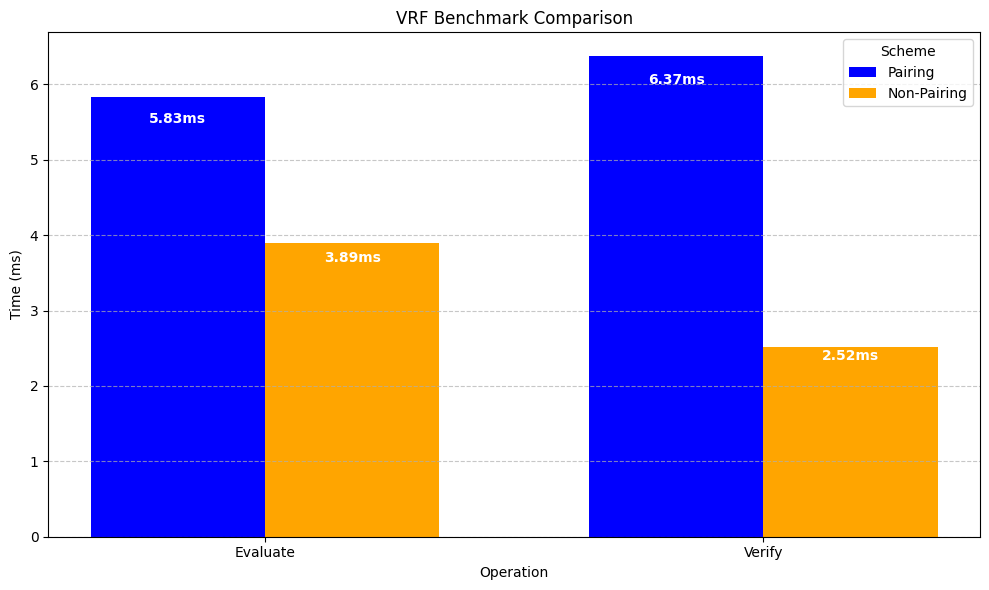
\includegraphics[width=0.75\linewidth]{figures/vrf-benchmark.png}
    \caption{VRF Benchmark}
    \label{fig:vrf-benchmark}
\end{figure}





\begin{table}[ht]
\begin{center}
\caption{Verification Time for 4 Credentials with Varying Attributes (time in ms)}
\label{tab:performance-vrf}
\begin{tabular}{l@{\hspace{1em}}r@{\hspace{2em}}r@{\hspace{5em}}r@{\hspace{2em}}r}
\toprule
\textbf{Scheme} & \multicolumn{2}{c}{\textbf{Eval + Prove (ms)}} & \multicolumn{2}{c}{\textbf{Verify (ms)}} \\
\cmidrule(lr){2-3} \cmidrule(lr){4-5}
& \textbf{ms} & \textbf{Speedup} & \textbf{ms} & \textbf{Speedup} \\
\midrule
DY$^1$ \cite{hutchison_verifiable_2005}                     & 1.27 &        & 2.2   &       \\
Our DY-PF \ref{sec-dy-pf}                                   & 0.41 & 3.1x   & 0.70  & 3.1x  \\
\midrule
DY Private \cite{tomescu2022utt}                            & 5.91 &        & 6.47  &       \\
Our DY-PF-Private \ref{sec-dy-pf-priv}                      & 1.08 & 5.5x   & 1.41  & 4.6x  \\
Our DY-PF-Private-ComOut \ref{sec-dy-pf-priv-com-out}       & 2.73 & 2.2x   & 2.07  & 3.1x  \\
\bottomrule
\end{tabular}
\par\medskip
\raggedright
\footnotesize{$^1$We use optimized pairing for verification by computing all pairings in Miller Loop format before a single Final Exponentiation, reducing verify time from 2.85(ms) to 2.27(ms), a 1.26x speedup.}

\footnotesize{$^2$[Your second footnote text here]} 
\end{center}
\end{table}



% implementation,operation,mean_ms
% dy,eval_prove,1.2868182107000956
% dy,verify_optimized,2.271014145714285
% dy,verify_standard,2.8528912494117655
% dy_pf,eval_prove,0.46260737338791946
% dy_pf,verify,0.7097862318577927


% dy_pf_priv,eval_prove,1.0801653887438827
% dy_pf_priv,Verify,1.4076584868270694



% dy_pf_priv_commited_output,eval_prove,2.7305393511111116
% dy_pf_priv_commited_output,verify,2.0714240844000003

% dy_priv,eval_prove,5.911952128888892
% dy_priv,verify,6.473554282857142




% \begin{table}
% \begin{center}
% \caption{Comparison of our construction over previous work.}
% \label{tab:comparison-chap4}
% \begin{tabular}{l|ccccc}
% Features    									& 
% Sybil Resist.  & 
% Hierarchy & 
% Private & 
% Pairing-Free & 
% Predicate Proofs \\
% \hline
% CanDID \cite{maram2021candid}     				&
% \ding{51}     & 
% \ding{51} 	& 
% \ding{55}  &  
% -     & 
% \ding{55}		\\
% SyRA \cite{crites_syra_2024}     				& 
% \ding{51}    	& 
% \ding{51}     & 
% \ding{51}  &  
% \ding{51}     & 
% \ding{55}		\\
% S3ID \cite{rabaninejad_attribute-based_2024}  & 
% \ding{51}     & 
% \ding{51}    	& 
% \ding{55}  &  
% \ding{55}     & 
% \ding{55}		\\
% UTT               & 
% \ding{51}     & 
% \ding{51}    	& 
% \ding{51}  &  
% \ding{55}     & 
% \ding{51}		\\
% Chap3             & 
% \ding{55}     & 
% \ding{55}    	& 
% \ding{51}  &  
% \ding{55}     & 
% \ding{51}		\\
% Ours  										& 
% \ding{51}     & 
% \ding{51}    	& 
% \ding{51}  &  
% \ding{51}     & 
% \ding{51}		\\
% \end{tabular}
% \end{center}
% \vspace{1em}
% \footnotetext[1]{Predicate Proofs allow users to prove statements about their credentials privately}
% \footnotetext[2]{Efficient Token refers to optimization of token verification}
% \end{table}
